\documentclass[sigconf,screen,review,anonymous]{acmart}

% Anonymous ACM double-column review manuscript.
\usepackage{amsmath}
\usepackage{booktabs}
\usepackage{graphicx}
\usepackage{microtype}
\usepackage{xcolor}

\definecolor{priorblue}{HTML}{2C7FB8}
\definecolor{modelorange}{HTML}{D95F0E}
\definecolor{calgreen}{HTML}{238B45}
\graphicspath{{figures/}}

% Compact float spacing without changing the ACM margins or type size.
\renewcommand{\topfraction}{0.95}
\renewcommand{\bottomfraction}{0.90}
\renewcommand{\textfraction}{0.05}
\renewcommand{\floatpagefraction}{0.80}
\setlength{\textfloatsep}{8pt plus 2pt minus 2pt}
\setlength{\floatsep}{8pt plus 2pt minus 2pt}

\setcopyright{none}
\settopmatter{printacmref=true,printfolios=true}
\acmConference[ACM MM '26]{Proceedings of the 34th ACM International Conference on Multimedia}{November 10--14, 2026}{Rio de Janeiro, Brazil}
\acmBooktitle{Proceedings of the 34th ACM International Conference on Multimedia (ACM MM '26), November 10--14, 2026, Rio de Janeiro, Brazil}
\acmYear{2026}
\acmDOI{}
\acmISBN{}
\hypersetup{pdfauthor={Anonymous Author(s)},pdftitle={Shared-Stimulus Structure Dominates Subject-Held-Out EEG--fNIRS Emotion Regression}}

\begin{document}

\title{Shared-Stimulus Structure Dominates Subject-Held-Out EEG--fNIRS Emotion Regression}

\author{Anonymous Author(s)}
\affiliation{%
  \institution{Anonymous Institution}
  \country{}
}
\email{}

\begin{abstract}
Continuous emotion regression estimates moment-to-moment valence and arousal
from physiological recordings. When every participant views the same
time-aligned videos, subject-held-out evaluation leaves stimulus identity and
time unchanged. Apparent accuracy may therefore reflect a stimulus-locked group
trajectory rather than information decoded from an individual's physiology.
We introduce a source-explicit decomposition that separates a fold-wise
video--time prior from an EEG--fNIRS predictor. Across 24 participants viewing
15 shared videos, the physiological branch obtained a mean absolute error
(MAE) of 47.3509, the prior 29.0633, and their fixed fusion 29.0146. An external
subject-disjoint evaluation on four viewers and 6,143 one-second samples further
separated a global constant, video identity, video--time dynamics, physiology,
and fusion, with MAEs of 44.3296, 33.3627, 28.0410, 42.7486, and 27.7246,
respectively. The aggregate fusion gain was heterogeneous, occurring in 3 of 4
viewers and 9 of 15 videos. Thus, video identity and within-video time explain
the main gains, while physiology provides a smaller, non-uniform residual
increment. This result does not imply that EEG or fNIRS lacks affective
information; it shows that subject-held-out evaluation alone cannot identify
its contribution when stimuli repeat. Source-explicit baselines and crossed
participant-by-stimulus splits are therefore necessary for interpretable
emotion regression.
\end{abstract}

\begin{CCSXML}
<ccs2012>
  <concept>
    <concept_id>10002951.10003260.10003277</concept_id>
    <concept_desc>Information systems~Multimedia information systems</concept_desc>
    <concept_significance>500</concept_significance>
  </concept>
  <concept>
    <concept_id>10010147.10010257.10010293.10010294</concept_id>
    <concept_desc>Computing methodologies~Neural networks</concept_desc>
    <concept_significance>300</concept_significance>
  </concept>
  <concept>
    <concept_id>10010405.10010444.10010450</concept_id>
    <concept_desc>Applied computing~Psychology</concept_desc>
    <concept_significance>300</concept_significance>
  </concept>
</ccs2012>
\end{CCSXML}

\ccsdesc[500]{Information systems~Multimedia information systems}
\ccsdesc[300]{Computing methodologies~Neural networks}
\ccsdesc[300]{Applied computing~Psychology}

\keywords{EEG--fNIRS, continuous emotion regression, shared-stimulus structure, video--time prior, subject-held-out evaluation}

\maketitle

\section{Introduction}
\label{sec:introduction}

Continuous emotion regression estimates moment-to-moment valence and arousal
while a viewer watches a video. Accurate group-level affect trajectories can
support video understanding and provide baselines for video editing,
advertising placement, content recommendation, or coarse initialization of a
new viewer's expected response. This paper focuses on the predictive
prerequisite for these uses: lowering mean absolute error (MAE) for new viewers
watching familiar, time-aligned videos.

EEG provides millisecond-scale electrophysiological measurements, whereas
functional near-infrared spectroscopy (fNIRS) captures slower haemodynamic
changes. Their complementary properties motivate EEG--fNIRS affect models
\cite{bandara2018fnirs,sun2020multimodal,chen2024eegfnirs}. Cross-participant
prediction nevertheless remains difficult because anatomy, sensor contact,
baseline state, and response style can produce shifts larger than the affective
variation of interest \cite{li2022eegreview,li2018crosssubject}. Collecting both
modalities from every new viewer also carries substantially greater sensing and
processing cost than using information already associated with the video.

The familiar-video setting changes what information is available. Naturalistic
movies can elicit time-locked inter-subject similarity in BOLD and EEG
responses
\cite{hasson2004intersubject,kauppi2010isc,dmochowski2012correlated}.
The reliability of these neural responses has been examined in relation to
emotion, attention, and audience preference
\cite{nummenmaa2012synchrony,ki2016attention,dmochowski2014audience}.
When training participants and a new viewer watch the same aligned video,
their matched labels permit a group affect trajectory indexed by video
identity and within-video time. A valid predictor must reconstruct this
trajectory inside each training split so that held-out labels cannot enter the
estimate.

We operationalize the shared response as a fold-wise video--time prior, pair it
with an EEG--fNIRS branch, and combine the two through prior-dominating fixed
fusion. The study is organized around three research questions:

\begin{description}
  \item[RQ1.] What MAE do the video--time prior and fixed fusion achieve when
  predicting new viewers' affect on familiar videos?
  \item[RQ2.] Which information source, global level, video identity,
  within-video time, or EEG--fNIRS, accounts for the MAE reduction?
  \item[RQ3.] How do the remaining gains vary across participants, videos, and
  within-video time?
\end{description}

Our contributions are threefold:

\begin{itemize}
  \item We formulate MAE-oriented continuous emotion prediction for new
  viewers of familiar videos and construct a fold-wise video--time prior that
  excludes labels from evaluated participants and has low marginal inference
  cost.
  \item We show empirically that the video--time prior is a strong predictor,
  while prior-dominating fusion with an EEG--fNIRS branch achieves the lowest
  evaluated MAE in both the internal subject-held-out and external
  subject-disjoint evaluations.
  \item We separate global level, video identity, within-video time, and
  EEG--fNIRS correction through source-explicit ablations and paired residual
  analysis, revealing a small and heterogeneous physiological contribution.
\end{itemize}

\section{Related Work}
\label{sec:related}

\subsection{Physiological emotion regression}

Physiological emotion recognition commonly represents affect in categorical or
valence--arousal spaces \cite{russell1980circumplex,koelstra2012deap}. EEG work
has identified informative spectral and spatial patterns
\cite{zheng2015critical}, while fNIRS studies use oxygenation-related statistics
to model affective state \cite{bandara2018fnirs}. Multimodal systems combine the
two signals through graph convolution, attention, or representation alignment
\cite{sun2020multimodal,chen2024eegfnirs,fang2026asac}. These mechanisms motivate
our EEG--fNIRS branch.

Cross-participant variation remains a persistent obstacle
\cite{li2022eegreview,li2018crosssubject}. Resting recordings and transfer
learning can align participants or personalize affective decoders
\cite{morioka2015resting,zheng2016personalizing}. Such methods address
participant shift, but they do not quantify the low-cost information already
contained in a familiar video's identity and playback time. A fair analysis of
this setting therefore requires an explicit video--time baseline beside the
physiological model.

\subsection{Naturalistic stimuli and shared responses}

Naturalistic movies can elicit time-locked inter-subject similarity in BOLD
and EEG responses
\cite{hasson2004intersubject,kauppi2010isc,dmochowski2012correlated}.
The reliability of these neural responses has been examined in relation to
emotion, attention, and audience preference
\cite{nummenmaa2012synchrony,ki2016attention,dmochowski2014audience}.
These studies establish shared stimulus-locked neural structure, but they do
not directly establish a continuous affect-label predictor.

In our repeated-stimulus setting, matched labels from training participants
permit a different operationalization: a fold-wise group trajectory indexed
by video identity and within-video time. The video--time prior turns this
trajectory into a low-cost regression baseline and directly compares it with
an EEG--fNIRS branch.

\subsection{Evaluation, priors, and leakage control}

Evaluation protocols determine which form of generalization a reported score
supports. Grouped cross-validation prevents direct participant overlap, but
repeated videos across folds still evaluate new participants on familiar
content \cite{saeb2017usecase,roberts2017crossvalidation}. Video-held-out and
crossed participant-by-video designs answer different questions. Model
selection within evaluation folds can further bias estimates
\cite{varma2006bias,varoquaux2017decoders}.

For familiar-video prediction, a video--time prior is legitimate only when it
is built from training participants and applied to identical held-out sample
keys. We therefore reconstruct the prior within every internal fold and keep
all external targets outside training and prior construction. Source-explicit
variants then separate the information supplied by global affect level, video
identity, within-video time, and EEG--fNIRS measurements.

\section{Method}
\label{sec:method}

\subsection{Problem formulation and pipeline}

For participant \(s\), familiar video \(v\), and second \(t\), the target is
\(y_{s,v,t}\in[1,255]^2\), containing valence and arousal. Our primary endpoint
is sample-pooled MAE over both affect dimensions,
\begin{equation}
 \operatorname{MAE} =
 \frac{1}{2N}\sum_{i=1}^{N}\sum_{d\in\{V,A\}}
 \left|y_i^d-\hat y_i^d\right|.
\end{equation}

The pipeline produces two complementary estimates before fusion. The
video--time prior \(\bar p_{v,t}\) retrieves the group trajectory associated with
the familiar video and second. The EEG--fNIRS branch \(m_{s,v,t}\) extracts
one-second channel features, encodes each modality with a graph network,
exchanges cross-modal information through attention, and regresses valence and
arousal from pooled tokens. A fixed convex combination returns the final
prediction \(\hat y_{s,v,t}\). This design makes the low-cost shared response and
the participant-specific physiological correction separately measurable.

\subsection{Fold-wise video--time prior}

Within each training fold, we aggregate labels at every video--time coordinate
using the cross-participant median:
\begin{equation}
 p^d_{v,t} =
 \operatorname{median}_{s\in\mathcal S_{\mathrm{tr}}} y^d_{s,v,t},
 \qquad d\in\{V,A\}.
\end{equation}
We then smooth each trajectory with a radius-three moving average,
\begin{equation}
 \bar p^d_{v,t} =
 \frac{1}{|\mathcal I_{v,t}|}
 \sum_{u\in\mathcal I_{v,t}} p^d_{v,u},
 \quad
 \mathcal I_{v,t}=\{u:|u-t|\leq3,\ 0\leq u<T_v\}.
\end{equation}
Smoothing never crosses video boundaries. The median limits the influence of
individual trajectories, and fold-wise reconstruction prevents held-out labels
from determining their own predictions. At inference, the prior is a lookup by
video identity and second, giving it low marginal input and computation cost
once the training trajectories have been built.

\subsection{EEG--fNIRS branch}

The EEG--fNIRS branch proceeds through channel-level feature extraction, graph
encoding within each modality, cross-modal attention in both directions, and
pooled regression. Signals are centred using the corresponding trial baseline, and
EEG is resampled to 200 Hz. For each EEG channel and one-second segment, we
compute relative log power and differential entropy in six bands from 1 to
45 Hz, together with Hjorth activity, mobility, and complexity
\cite{hjorth1970eeg}. Concatenating the features from \(t-1\), \(t\), and
\(t+1\) yields a \(64\times45\) EEG tensor.

For each fNIRS channel and each of six signal types, we compute mean, standard
deviation, slope, skewness, and kurtosis. The same three-segment concatenation
yields a \(51\times90\) fNIRS tensor. Edge padding is used at trial boundaries.
Because both tensors include the \(t+1\) segment, the branch is an offline
estimator rather than a strictly causal real-time decoder.

Each modality is encoded with a learned-adjacency, multi-order graph network
using identity, first-order, and second-order propagation supports. The encoder
produces 32-dimensional channel embeddings. Four-head attention exchanges
information in the EEG-to-fNIRS and fNIRS-to-EEG directions
\cite{vaswani2017attention,tsai2019multimodal}. Mean and maximum pooling over
modality-specific and cross-modal tokens feed a multilayer regressor. Training
minimizes normalized-target mean squared error plus \(0.01\) times a symmetric
contrastive alignment loss \cite{chen2020simclr}. The alignment term regularizes
paired EEG and fNIRS representations from the same sample without dominating
the regression objective. Models use participant-grouped folds, AdamW
optimization, strong dropout, and early stopping on fold validation MSE.

\subsection{Prior-dominating fixed fusion}

The final estimate is
\begin{equation}
 \hat y_{s,v,t}
 = w\odot \bar p_{v,t} + (1-w)\odot m_{s,v,t},
 \qquad w=[0.99,0.92].
\end{equation}
The fixed weights intentionally keep the video--time prior dominant for valence
and arousal. Our objective is to test whether EEG--fNIRS can provide residual
correction to an already strong low-cost estimate, rather than to optimize a
complex adaptive gating model. The same weights are used for every split and
both evaluations, which makes the incremental correction directly
interpretable.

\section{Experimental Setup}
\label{sec:setup}

\subsection{Dataset and participants}

The development dataset contains 24 participants, 15 familiar videos viewed by
all participants, 360 trials, and 36,864 one-hertz valence--arousal targets
\cite{merpsdataset}. Each trial includes a five-second resting baseline. EEG
contains 64 channels, and fNIRS contains six signal types over 51 channels.
Targets and predictions remain on the original \([1,255]\) scale.

\subsection{Internal subject-held-out evaluation}

Participants are partitioned into five folds. For each fold, the video--time
prior is reconstructed only from training participants, and the matching
EEG--fNIRS checkpoint predicts the held-out participants. The full-data
checkpoint is excluded. Predictions and targets from all folds are concatenated
before computing sample-pooled overall, valence, and arousal MAE. This protocol
evaluates new viewers responding to the same 15 familiar videos.

\subsection{External subject-disjoint evaluation}

The external cohort contains four participants, 60 trials, and 6,143 one-hertz
targets. These participants are disjoint from the development set. Their targets
are excluded from prior construction, checkpoint training, and inference, and
are joined to predictions only for local evaluation. The external EEG--fNIRS
estimate averages one fixed-split checkpoint and five participant-grouped fold
checkpoints. Fixed fusion combines this ensemble with a video--time prior built
from all 24 development participants.

\subsection{Source variants}

Table~\ref{tab:source-variants} summarizes the information used by each
variant at inference. The label-aggregate column denotes direct lookup of a
cached statistic computed from development-participant labels; evaluated
participants are excluded from these aggregates.

\begin{table}[H]
  \caption{Information used by each source variant at inference. The label
  aggregate is computed from development-participant labels; all physiological
  models are nevertheless trained on development targets.}
  \label{tab:source-variants}
  \centering
  \scriptsize
  \setlength{\tabcolsep}{3.1pt}
  \begin{tabular}{@{}lcccc@{}}
    \toprule
    Variant &
    \shortstack{Participant\\phys.} &
    \shortstack{Video\\key} &
    \shortstack{Time\\key} &
    \shortstack{Label\\agg.} \\
    \midrule
    Global constant & N & N & N & Y \\
    Video identity & N & Y & N & Y \\
    Video--time prior & N & Y & Y & Y \\
    EEG--fNIRS branch & Y & N & N & N \\
    Fixed fusion & Y & Y & Y & Y \\
    \bottomrule
  \end{tabular}
\end{table}

The global constant is the two-dimensional median over all development labels.
The video-identity variant uses the temporal median of each development video
trajectory and remains constant within that video. The video--time prior uses
the full median trajectory with radius-three within-video smoothing. The
EEG--fNIRS and fixed-fusion variants follow Section~\ref{sec:method} and the
external ensemble definition above. The internal archive contains the final
three variants; the external evaluation contains all five.

\subsection{Metrics and reporting}

We report sample-pooled MAE overall and separately for valence and arousal on
identical prediction keys. Overall MSE is retained as a secondary external
diagnostic, while MAE remains the primary endpoint. For external heterogeneity
analysis, paired errors are also aggregated by participant, by familiar video,
and by ten equal bins of normalized within-video time. These grouped summaries
are descriptive because the external cohort is small and adjacent one-second
targets are temporally correlated. The internal archive contains aggregate
component metrics rather than paired sample-level residuals.

\section{Results and Analysis}
\label{sec:results}

\subsection{RQ1: Main MAE performance}

Table~\ref{tab:main-mae} combines the internal and external results. Fixed
fusion achieved the lowest overall MAE in both evaluations, reaching 29.01
internally and 27.72 externally. The video--time prior stayed within 0.05 and
0.32 MAE, respectively, whereas the EEG--fNIRS branch was substantially less
accurate. Valence and arousal followed the same ordering.

\begin{table*}[t]
  \caption{Internal and external MAE on the original label scale. Lower is
  better; dashes mark source variants unavailable in the internal archive.}
  \label{tab:main-mae}
  \centering
  \small
  \setlength{\tabcolsep}{6pt}
  \renewcommand{\arraystretch}{1.08}
  \begin{tabular}{@{}llrrrrr@{}}
    \toprule
    Evaluation & Target & Global & Video ID & Video--time prior & EEG--fNIRS & Fusion \\
    \midrule
    Internal & Overall & -- & -- & 29.06 & 47.35 & \textbf{29.01} \\
             & Valence & -- & -- & 26.67 & 51.35 & \textbf{26.66} \\
             & Arousal & -- & -- & 31.46 & 43.35 & \textbf{31.37} \\
    \midrule
    External & Overall & 44.33 & 33.36 & 28.04 & 42.75 & \textbf{27.72} \\
             & Valence & 47.46 & 32.56 & 25.34 & 45.29 & \textbf{25.20} \\
             & Arousal & 41.20 & 34.17 & 30.74 & 40.21 & \textbf{30.25} \\
    \bottomrule
  \end{tabular}
\end{table*}

\begin{figure}[t]
  \centering
  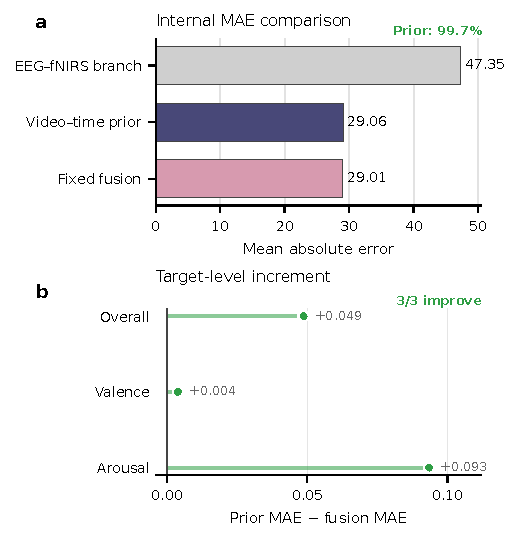
\includegraphics[width=\columnwidth]{source_dominance.pdf}
  \caption{Internal subject-held-out MAE. (a) Overall MAE for the EEG--fNIRS
  branch, video--time prior, and fixed fusion. (b) Additional MAE reduction
  from the prior to fusion by target.}
  \Description{A two-panel figure compares overall internal MAE and the small
  additional reduction from the video--time prior to fixed fusion.}
  \label{fig:source-dominance}
\end{figure}

Figure~\ref{fig:source-dominance} shows the same internal pattern visually. The
large reduction from the EEG--fNIRS branch to the final predictor was almost
entirely recovered by the video--time prior, while fusion supplied the smallest
final step.

\subsection{RQ2: Source decomposition}

The staged external variants identify the source of the reduction. Replacing
the global constant with video identity lowered overall MAE by 10.97 points;
adding within-video time lowered it by a further 5.32 points. The shared
response therefore contains both a video-specific affect level and a
substantial time-resolved trajectory.

Across the full path from the EEG--fNIRS branch to fixed fusion, the video--time
prior accounted for 99.73\% of the internal reduction and 97.89\% of the external
reduction. The fixed fusion remained best, but most of its advantage over the
EEG--fNIRS branch was already available from video identity and within-video
time. Figure~\ref{fig:external-decomposition}a shows the complete external
ordering of the five variants.

\begin{figure*}[t]
  \centering
  
\includegraphics[width=\textwidth]{external_source_decomposition.pdf}
  \caption{External MAE and residual analysis. (a) Overall MAE for five source
  variants. (b,c) Participant- and video-level prior-minus-fusion increments;
  positive values favour fusion. (d) MAE over normalized video-time bins.}
  \Description{A four-panel figure shows external overall error, paired
  participant- and video-level fusion increments, and error over normalized
  video time.}
  \label{fig:external-decomposition}
\end{figure*}

\subsection{RQ3: Heterogeneity across participants, videos, and time}

The external residuals show that the EEG--fNIRS correction was not uniform.
Fusion lowered MAE for 3 of 4 participants and 9 of 15 familiar videos
(Figure~\ref{fig:external-decomposition}b,c). Participant-level changes ranged
from a 0.06-point worsening to a 0.69-point improvement. Video-level changes
ranged from a 0.30-point worsening to a 1.31-point improvement. The lower
aggregate fusion MAE therefore coexisted with localized gains and losses.

The contribution of within-video time also varied across a video
(Figure~\ref{fig:external-decomposition}d). In the first normalized time bin,
video identity reached 45.53 MAE and the video--time prior reached 13.40. This
advantage narrowed over time, and video identity was slightly better in each of
the final five bins. The aggregate temporal gain was therefore concentrated in
specific phases rather than distributed uniformly.

\section{Discussion and Limitations}
\label{sec:discussion}

\subsection{Why the video--time prior is effective}

The video--time prior is effective because the deployment setting preserves two
strong coordinates: familiar video identity and playback time. Participants
respond differently, but a shared audiovisual sequence still induces a
population-level trajectory. Median aggregation limits individual extremes,
and within-video smoothing reduces local variation without crossing video
boundaries. The resulting predictor gains its strength from the data structure
rather than from model complexity.

This property gives the prior practical value. Once previous viewers have
established a trajectory, a new viewer can receive a low-cost approximate curve
without EEG or fNIRS acquisition. Such curves may serve as group-response
baselines for video editing, advertising placement, content recommendation, or
initialization of a new viewer's expected response.

\subsection{When EEG--fNIRS adds value}

EEG--fNIRS is most useful when participant-specific deviations from the group
trajectory are both measurable and stable. The external residuals indicate
that this condition held for some participants and videos but not for all of
them. This heterogeneity makes sensing cost part of the design decision:
fusion offers the lowest aggregate MAE, whereas the prior supplies most of the
benefit without new physiological measurement.

Several mechanisms could limit the correction, including sensor noise,
handcrafted one-second features, imperfect haemodynamic timing,
cross-participant shift, and a model that does not explicitly isolate residuals
from the prior. The present analysis locates gains and losses but does not
distinguish among these explanations. Future work should test stronger residual
modelling and explicit haemodynamic alignment.

\subsection{Implications for practice and evaluation}

The results also clarify the evaluation question. Subject-held-out evaluation
with familiar videos measures generalization to new participants, whereas
video-held-out evaluation measures transfer to new content. Future studies
should separate these axes through crossed participant-by-video splits and
rebuild the prior, feature standardization, checkpoint selection, and fusion
weights within each outer training split
\cite{varma2006bias,varoquaux2017decoders}. Participant-macro, video-macro, and
paired residual summaries would further preserve the hierarchy hidden by a
single sample-pooled score.

For deployment, the choice between the prior and fusion depends on the value of
the residual improvement relative to acquisition cost. The prior provides a
simple group baseline for familiar content, while EEG--fNIRS can be reserved
for settings in which participant-specific correction is worth the additional
instrumentation.

\subsection{Limitations and future work}

The conclusions are bounded by the familiar-video setting: all participants
viewed the same 15 videos, so transfer to unseen content was not measured. The
external cohort contains only four participants, and adjacent one-second
targets are correlated; its heterogeneity analysis is therefore descriptive
rather than stable participant-level inference. Fusion weights and checkpoint
choices were not selected through a fully nested procedure, and the internal
and external fusion increments are not directly comparable because their
physiological ensembles and held-out groups differ. The EEG--fNIRS branch uses
one-second future context and no explicit fNIRS haemodynamic shift, so it is an
offline estimator. The study evaluates prediction error rather than downstream
application utility. Anonymous identifiers prevent demographic or subgroup
analysis, and the physiological architecture represents one comparator.
Crossed participant-by-video evaluation, nested selection, and stronger
residual modelling are the main priorities for broader validation.

\section{Conclusion}
\label{sec:conclusion}

This work establishes a fold-wise video--time prior that excludes evaluated
participants' labels as a strong, low-cost baseline for continuous emotion
regression on familiar videos. Fixed
fusion with an EEG--fNIRS branch achieved the lowest MAE in both internal and
external evaluations, but source decomposition showed that video identity and
within-video time supplied most of the reduction. EEG--fNIRS provided a smaller
and heterogeneous residual correction. The approach can support group-response
curves when familiar content is available, while broader claims require crossed
participant-by-video evaluation and nested residual-model selection.


\clearpage
\bibliographystyle{ACM-Reference-Format}
\bibliography{references}

\end{document}
